Generally, we developed the system which we used to achieve our senior design 
project, and we drew the block diagram to delineate the subsystems and individual
tasks, which is shown as Figure \ref{fig:block_diagram}.The system is composed of 
four main modules: Control Module, Actuator Module, User Interaction Module, and 
Power Module, collaboratively enabling a VR-guided robotic claw system with closed-loop force control and CAN communication.
\begin{figure}[h]
    \centering
    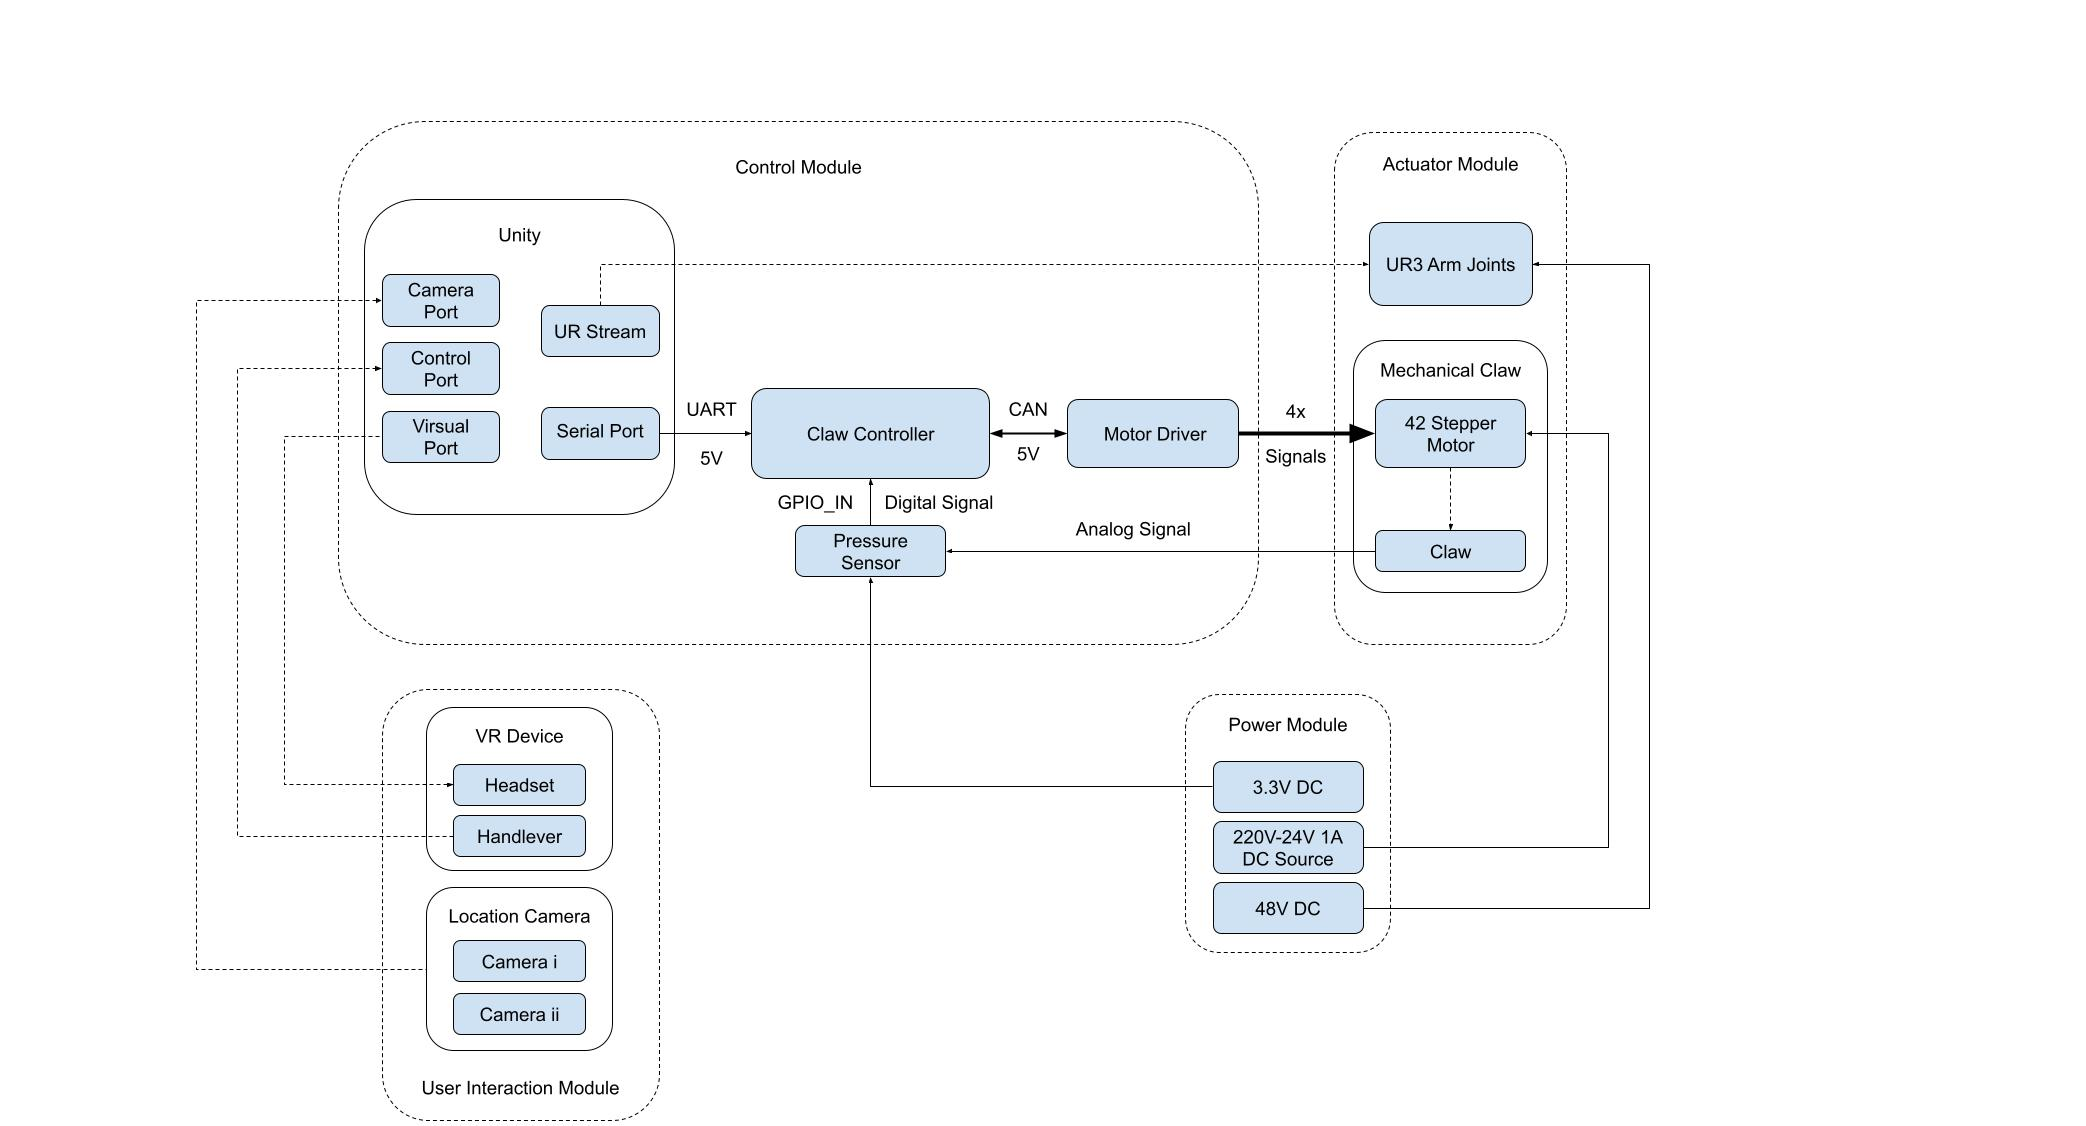
\includegraphics[width=0.8\textwidth]{Figures/Block Diagram 2.0.jpg}
    \caption{Block Diagram}
    \label{fig:block_diagram}
\end{figure}
\subsection*{Control Module}
At the core of the system lies the Control Module, where Unity software runs and interfaces with the physical system via multiple communication ports. The UR Stream and Serial Port in Unity handle command and signal exchange through UART with the Claw Controller (based on an STM32 microcontroller). The controller processes incoming signals and sends control commands via CAN bus to the Motor Driver, which in turn drives the 42 Stepper Motor. Additionally, a Pressure Sensor provides real-time feedback to the Claw Controller via analog and GPIO inputs, forming a basic closed-loop control system for grasping force regulation.
\subsection*{Actuator Module}
The Actuator Module consists of a 42 Stepper Motor and a 3D-printed claw. The motor is controlled by the Motor Driver, which receives commands from the Claw Controller via CAN bus. The claw's design allows for precise control of the grasping force, enabling the system to adapt to various objects and scenarios.
\subsection*{User Interaction Module}
The User Interaction Module is designed to facilitate user engagement with the system. It includes a VR headset and controllers, which provide an immersive experience for the user. The Unity software processes input from the VR controllers and translates it into commands for the Claw Controller, allowing users to interact with virtual objects in a realistic manner.
\subsection*{Power Module}
The Power Module supplies the necessary power to the entire system. It ensures that all components, including the Control Module, Actuator Module, and User Interaction Module, receive stable and sufficient power for optimal performance.
  
Initially, we planned to use a STM32F103 microcontroller and SG-90 motor to control the claw. However, we found the accuracy was low and reaction time was far from satisfactory. Therefore, we changed to use more powerful STM32F407 with M4 core and 42 stepper motor. In addition, we wanted to use unity to control arm through ROS system at first, but we finally found a online source which allowed us to control arm derectly by unity hub, which reduces the complexity and optimizes the performance of the system.